\section{W5: Agile Estimations and Planning}

\textbf{1. Understand Agile SDLC Planning and Estimation Techniques.}

\textbf{2. Requirement gathering in Traditional and Agile.}
    \textbf{2.1. User Stories}: characteristics follow INVEST (Independent, Negotiable, Valuable, Estimable, Small, Testable).

    \textbf{2.2. Epics}: large user stories that cannot be completed in a single iteration.

    \textbf{2.3. Acceptance Criteria (AC's)}: conditions that a software product must satisfy to be accepted by a user, customer, or other stakeholders.

    \textbf{2.4. Definition of Done (DoD)}: a shared understanding of what it means for work to be complete.



\textbf{3. Scrum Artefacts.}

\textbf{4. Agile Estimations.}

    \textbf{4.1. Velocity}: measure of the amount of work a team can tackle during a single sprint. V = \# of team members * SP per day * \# of days in sprint.

\textbf{5. Agile Planning.}

    \textbf{5.1. MoSCoW}: Must have, Should have, Could have, Won't have.

    \textbf{5.2. Planning Artefacts}
    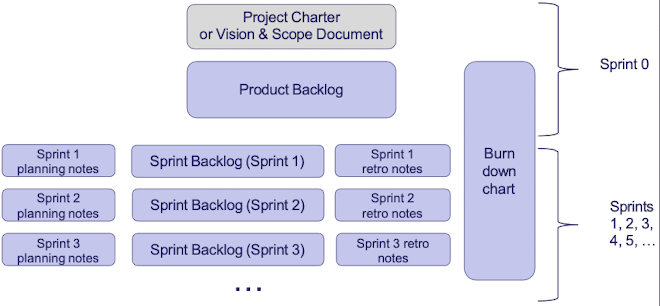
\includegraphics[width=\linewidth]{figs/SCR-20240606-lcfi.png}
